% status: 100 
% chapter: REST

\def\paperstatus{100} % a number from 0-100 indicating your status. 100
                % means completed
\def\paperchapter{REST} % This section is typically a single keyword. from
                   % a small list. Consult with theinstructors about
                   % yours. They typically fill it out once your first
                   % text has been reviewed.
\def\hid{hid-sp18-415} % all hids of the authors of this
                                % paper. The paper must only be in one
                                % authors directory and all other
                                % authors contribute to it in that
                                % directory. That authors hid must be
                                % listed first
\def\volume{9} % the volume of the proceedings in which this paper is to
           % be included

\def\locator{\hid, Volume: \volume, Chapter: \paperchapter, Status: \paperstatus. \newline}

\title{Linear Regression REST Service and API}



\author{Janaki Mudvari Khatiwada}
\affiliation{%
  \institution{Indiana University}  
  \city{Bloomington} 
  \state{IN} 
  \postcode{47408}
  \country{USA}}
\email{janu.khatiwada@gmail.com}


% The default list of authors is too long for headers}
\renewcommand{\shortauthors}{J. M. Khatiwada}



\begin{abstract}
  Python's flask application requires minimal application for application
  development. Flask make use of backend data as a resource to support an
  application running on the server. This project discusses development
  and deployment of REST api with python flask. This flask api gets current
  details
  info based on regression model created from car dataset. Once flask app runs 
  successfully, it is then deployed to Heroku, a platform as a service 
  cloud platform. For the purpose car data set from UCI machine learning
  data repository is being used. Before this, a regression model for the
  data has to be built to make sure that this model best describes the 
  relationship between variables, in this case engine size and highway
  miles per gallon. Based on this model new data set can be tested to make 
  prediction. Then regression results is used as the endpoint 
  in flask api. This service is then tested by running dockerfile.
   
\end{abstract}

\keywords{\locator\ Flask, Cloud Computing, Regression Model}


\maketitle

\section{Introduction}
Flask is a web application framework ``based on the Werkzeug WSGI (Web Server
Gateway Interface) toolkit and Jinja2 template 
engine''~\cite{hid-sp18-415-flask}. Being an interface between web server
and and web applications, ``it implements requests and response objects'' 
while jinja2 render web page by combining template and data 
source~\cite{hid-sp18-415-www-flask}. 
Flask api framework requires minimal framework for RESTful web services.
Rest services is an architectural style web services which use HTTP protocol
to establish communication between client and server during each service
request.
Being lightweight and scalable, flask is chosen as a good option for 
developing the RESTful apis. While flask does not have built--in support for 
database handling and validation support, these functionality can be added as
extensions to the application~\cite{hid-sp18-415-www-flask}.
The main purpose of this paper is
to create a regression model for car data set and then create a web service
with flask. The model is intended to
predict highway miles per gallon based on engine size of the vehicle.
Scikit-learn is used to run simple linear regression and build the prediction
model. This model is going
to be the resource in flask api. Using GET and POST methods to call
endpoints. GET method fetch resource info while POST method creates
a new resource. Resources and requests for API can be in different data
format but json format
is easy to understand and flask has in--built support for this data format. So 
our resource will be our json object stored in key--value pair.
  
Once flask api is succesfully run in localhost, the application is
then deployed to heroku which is an open source platform as a 
service cloud platform. This also has a minimal deployment needs.
It requires opening an account in heroku.com, then download heroku
command line interface (CLI). Then run heroku login from CLI and
and create an app. This flask appplication is about running machine learning
learning algorithm in heroku. It requires python packages such as pandas and 
scikit--learn, we deploy our app by packaging all required packages in docker
container and pushed to the platform. This process is discussed in more detail 
under \textit{methods} section.
  
\section{Simple Linear Regression}

  Just to provide a brief overview of why simple linear regression is
  chosen for the project, a brief introduction about it would be
  appropriate. Linear Regression is a statistical data analysis tool
  which describes the effect of one variable, also called independent
  variable, on dependent variable. In case of simple linear regression
  there is only one dependent variable with one independent variable.
  Our purpose of running this project
  is to create a line of best fit model to build a model that can be used
  for prediction. In this case prediction of mpg based on engine size
  of the vehicle. The line of best fit is described by the
  formula \[y = a + bx\] where a is coefficient or y intercept and b is
  slope for the line. In this case formula for prediction model or
  regression is given below, where \verb|hwy\_mpg| is y variable and
  \verb|engine\_size| is x variable.
  \[hwy\_mpg = yintercept + slope.enginesize\] 

\section{Methods}
 
  Data selection, cleaning and preprocessing, building a local
  environment, building a linear regression model using SciKit--learn,
  designing a REST api with Flask. The application is then tested by running 
  locally and also deploying it into heroku are the main
  processes of this project. They are explained below in details. 

   Automobile Data Set, \textit{https://archive.ics.uci.edu/ml/
   machine--learning-databases/autos/imports--85.data}, from UCI
   Machine learning data repository is selected. It was created
   on 19 May, 1987 by Jefferey C. Schlimmer~\cite{hid-sp18-415-uci-com}. The
   data set is multivariate with 25 attributes. Since the project
   is focused on designing and deploying a simple linear
   regression api as a demonstration of implementing Flask service,
   only two attributes, `engine size' and `highway miles per gallon'
   are used. Rest of the attributes are dropped. The goal of the
   project is to build a best fit prediction model for highway mpg
   based on engine size. The data set have several missing instances
   as well which are removed as a clean up process. Cleaned data is stored in
   Dropox as a csv   file so that it can be easily fetched into the
   application~\cite{hid-sp18-415-data}.
  
 Ubuntu 16.04 is the operating system used for whole project.
 A virtual environment pyenv is created in Ubuntu 16.04 where python 3
 environment is built. Besides, flask, this project requires different python
 packages to fetch and manipulate data and run the linear regression and
 then build a flask api. Using pip install package name, packages Flask,
 pandas, numpy, scipy and SciKit--learn are installed. Besides these
 packages, python packages matplotlib and seaborn are also installed as they
 are required to create a regression plot and plot line of best fit. 
 
 Once environment is setup regression or prediction model needs to be build
 from the data set so that this model is used in Flask app. This is done by
 running python's machine learning application. There are two types of
 machine learning, supervised and unsupervised learning. Supervised
 Machine learning is learning properties of data set (training data set)
 and applying them to the test data set. This machine learning algorithm
 is also called supervised learning. Regression problem in Scikit--learn
 is supervised machine learning. In this case predicting highway mpg for
 the new data set based on engine size is the regression problem. Data
 is split into train set and test set in 2:8 ratio.
    
 Regression analysis or building a best fit model for our data set is
 discussed in detail under section Analysis and Algorithm. Now the data
 set is split into two sets one used for defining a regression 
 equation. This equation is going to be the prediction model for data.
 Once regression equation is defined
 that is value for slope and intercept is calculated.   
 Source codes are located in github repository~\cite{hid-sp18-415-regression}.
   
The final process is writing a flask api which can be run to call 
endpoints using `GET' and `POST' methods. In this project predict is the
endpoint for POST method and and current details is the endpoint for GET
method. Then this application is deployed into heroku cloud platform from
CLI. Before deploying `heroku create app--name' is run to create an app within
heroku. Then run `git init' to initiate a remote git repository, since app is 
deployed through git push. In order to deploy to heroku it needs `Procfile'
with the process it needs to run and requirements.txt or Pipfile that has lists 
of dependencies needed for the app. Since this api needs to run regression, all
the needed packages numpy, scipy, pandas and scikit--learn are configured from 
Dockerile. For a minimal flask deployment following commands are run 
`git remote', `git add' to add files, `git commit' and `git push heroku master'.
In this case app is pushed using docker container for simplification.    

\section{Analysis and Algorithms}

 The cleaned data set has two attributes \textit{engine size} and
 \textit{highway miles per gallon} and 199 data points. Before developing
 a flask api, a linear regression machine learning model is created using
 scikit-learn. As discussed earlier this is going to be the prediction model
 and one of the endpoints for flask api.

 As it is mentioned above data set is split into two, one is train
 set and other is test set using algorithm train\_set\_split. 
 Train--set data is used to build the regression
 model. In order to train data set, we move label column to its own data frame
 called `train\_labels by pulling  series``hwy\_mpg'' from 
 train--set~\cite{hid-sp18-415-regression}. Then `LinearRegression' 
 class is created and fit 
 method is called by \[lin\_reg = LinearRegression()\] 
 \[lin\_reg.fit(train\_set, train\_labels)\]. Now we calculate intercept and
 slope our model. These values are used to create model formula
 as discussed in linear regression section above. Then predict function is
  called  by passing series test\_set which returns an array of predicted 
  values~\cite{hid-sp18-415-regression}. This model can be checked by calling
  print function for hwy\_mpg\_pred
  and test\_set series and compare values for each series. Another method to
  check how significant the model is by calculating the value for r--square 
  which in this case is lin\_reg score by running following algorithm.  
  \[lin\_reg.score(test\_set, test\_set\_full[`hwy\_mpg'])\]
  The value of this score ranges between 0 to 1. R square is called coefficient
  of determination. R square means that all the data points of the model falls
  perfectly on regression line. If value is more towards 0 then the regression 
  line far away from the data points and model is not a good fit for the data
  set. For the created model of this analysis r square value is 
  0.584835 can be rounded to 0.585.
  
  After defining the model flask api is developed where just created model will 
  be the resource object. The application file is located in github 
  repository~\cite{hid-sp18-415-regressionapi}. But before this,
  we should make sure the model do not 
  change when new data points are added. For the purpose joblib is being used.
  handle arrays stored in the models. Joblib persists newly created
  scikit--learn model so that for future use the model does not need to be
  retrained~\cite{hid-sp18-415-joblib}. Function joblib.load is being used in
  the application to load pickled regression model. This api calls one resource 
  current--details  and post predict value of hwy\_mpg when value for engine
  size is entered. 
   
  
\section{Regression Results}

 R square value shows how likely that predicted highway mpg fits into the
 regression model. It is 58 percent likely that future prediction will fall
 on the best fit line. It can be concluded that the model is fairly fit. While 
 58 percent of variance in highwaympg can be explained by engine size,
 there is 42 percent unexplained
 variance in highway mpg. To compare real highway miles per gallon values with 
 predicted values, print function is
 run for test\_set and hwy\_mpg\_pred set.
 
 Results can be compared between Table~\ref{tab:PredMPG} 
 and Table~\ref{tab:TestSetMPG}. 
 The first Table~\ref{tab:TestSetMPG} lists highway mpg with engine size 
 from our test\_set data. Just looking at the table we can see negative 
 relationship between engine size and highway mpg. 
 
 \begin{table}[htb]
  \centering
   \begin{tabular}{|c|c| p{5cm}|}
   \hline{}
    engine\_size & hwy\_mpg \\ 
    \hline
     82  & 32 \\ 
     \hline
     15  & 22 \\ 
     \hline
     111 & 25 \\ 
     \hline 
     177 & 34 \\ 
     \hline
     76  & 30 \\ 
     \hline
     163 & 30 \\ 
     \hline
     68  & 18 \\ 
     \hline
     67  & 25 \\ 
     \hline
     120 & 30 \\ 
     \hline
     173 & 24 \\ 
     \hline
     176 & 46 \\ 
     \hline
     148 & 32 \\ 
     \hline
     65  & 25 \\ 
     \hline
     30  & 38 \\ 
     \hline
     86  & 37 \\ 
     \hline
     85  & 30 \\ 
     \hline
     55  & 23 \\ 
     \hline
     60  & 42 \\ 
     \hline
     90  & 37 \\ 
     \hline
     159 & 29 \\ 
     \hline
     16  & 20 \\ 
     \hline
     124 & 25 \\ 
     \hline
     96  & 34 \\ 
     \hline
     172 & 24 \\ 
     \hline
     66  & 25 \\ 
     \hline
     189 & 28 \\ 
     \hline
     147 & 37 \\ 
     \hline
     9   & 29 \\ 
     \hline
     18  & 43 \\ 
     \hline
     128 & 28 \\ 
     \hline
     190 & 28 \\ 
     \hline
     45  & 19 \\ 
     \hline
     192 & 22 \\ 
     \hline
     164 & 30 \\ 
     \hline
     101 & 25 \\ 
     \hline
     69  & 18 \\ 
     \hline
     126 & 28 \\ 
     \hline
     123 & 25 \\ 
     \hline
     75  & 38 \\ 
     \hline
     78  & 32 \\ 
     \hline
   \end{tabular}  
   \caption{Highway MPG for Each Engine Size From Test Dataset} 
   \label{tab:TestSetMPG}
\end{table}

 while Table~\ref{tab:PredMPG} shows an array of 
 predicted highway mpg. 
 
 \begin{table}[htb]
\resizebox{\columnwidth}{!}{%
    \begin{tabular}{llcrrp{8cm}}
    \hline
    \midrule
    \multicolumn{3}{c}{Array of hwy\_mpg\_pred}\\ 
    \hline
  31.18833214 & 21.44002624 & 27.82684735 & 32.64497555 &  33.87751997 \\						
  28.4991443  &  18.63878892 & 24.35331306 & 31.18833214 & 25.69790698 \\						
  33.98956946 & 34.54981693 & 24.35331306 &  34.54981693 & 33.98956946 \\						
  32.53292605 & 35.89441084 & 31.18833214 &  33.98956946 & 33.87751997 \\						
  21.44002624 & 23.12076864 & 31.41243112 & 25.69790698 & 24.35331306 \\						
  29.05939177 & 34.54981693 & 32.75702504 & 34.77391591 & 31.30038163 \\						
  29.05939177 & 15.94960108 & 30.29193619 & 28.4991443  & 24.57741205 \\						
  18.63878892 & 31.30038163 & 23.12076864 & 34.54981693 & 31.18833214 \\
  \hline
  \midrule
    \end{tabular}
}
    \caption{Array of Predicted Highway MPG from  Model}
    \label{tab:PredMPG}
\end{table}
 
 Looking at both tables the predicted values while 
 not exactly same as observed values are quite similar to observed values 
 from test dataset. If predicted output are exactly similar to that of 
 observed then this would have been a 
 perfectly fit model with all data points from test\_set passing through the
 line of regression plot from model with r--square value equal to 1.
 The whole output can be found in github~\cite{hid-sp18-415-analysis}.
 It shows that values are pretty close.
 
 Another way to check how good or accurate the model is by plotting regression 
 plot from from model over scatter plot from test set. 
 Figure~\ref{fig:regplt}. The figure below shows a regression plot
 over scatterplot. The regression plot from original data shows the variability
 in observed values of highway mpg is explained by the independent variable.
 
 \begin{figure}[!h]
  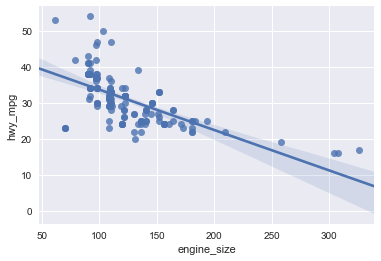
\includegraphics[width=\columnwidth]{images/reg_plot.png}
  \caption{Regresssion Plot Engine size and Highway MPG}
\label{fig:regplt}
\end{figure}
 
 
 Regression plot from model as seen in Figure~\ref{fig:predplt} shows 
 the regression line or line of best fit passes nearby most of the data
 points. 
 
 \begin{figure}[htb]
  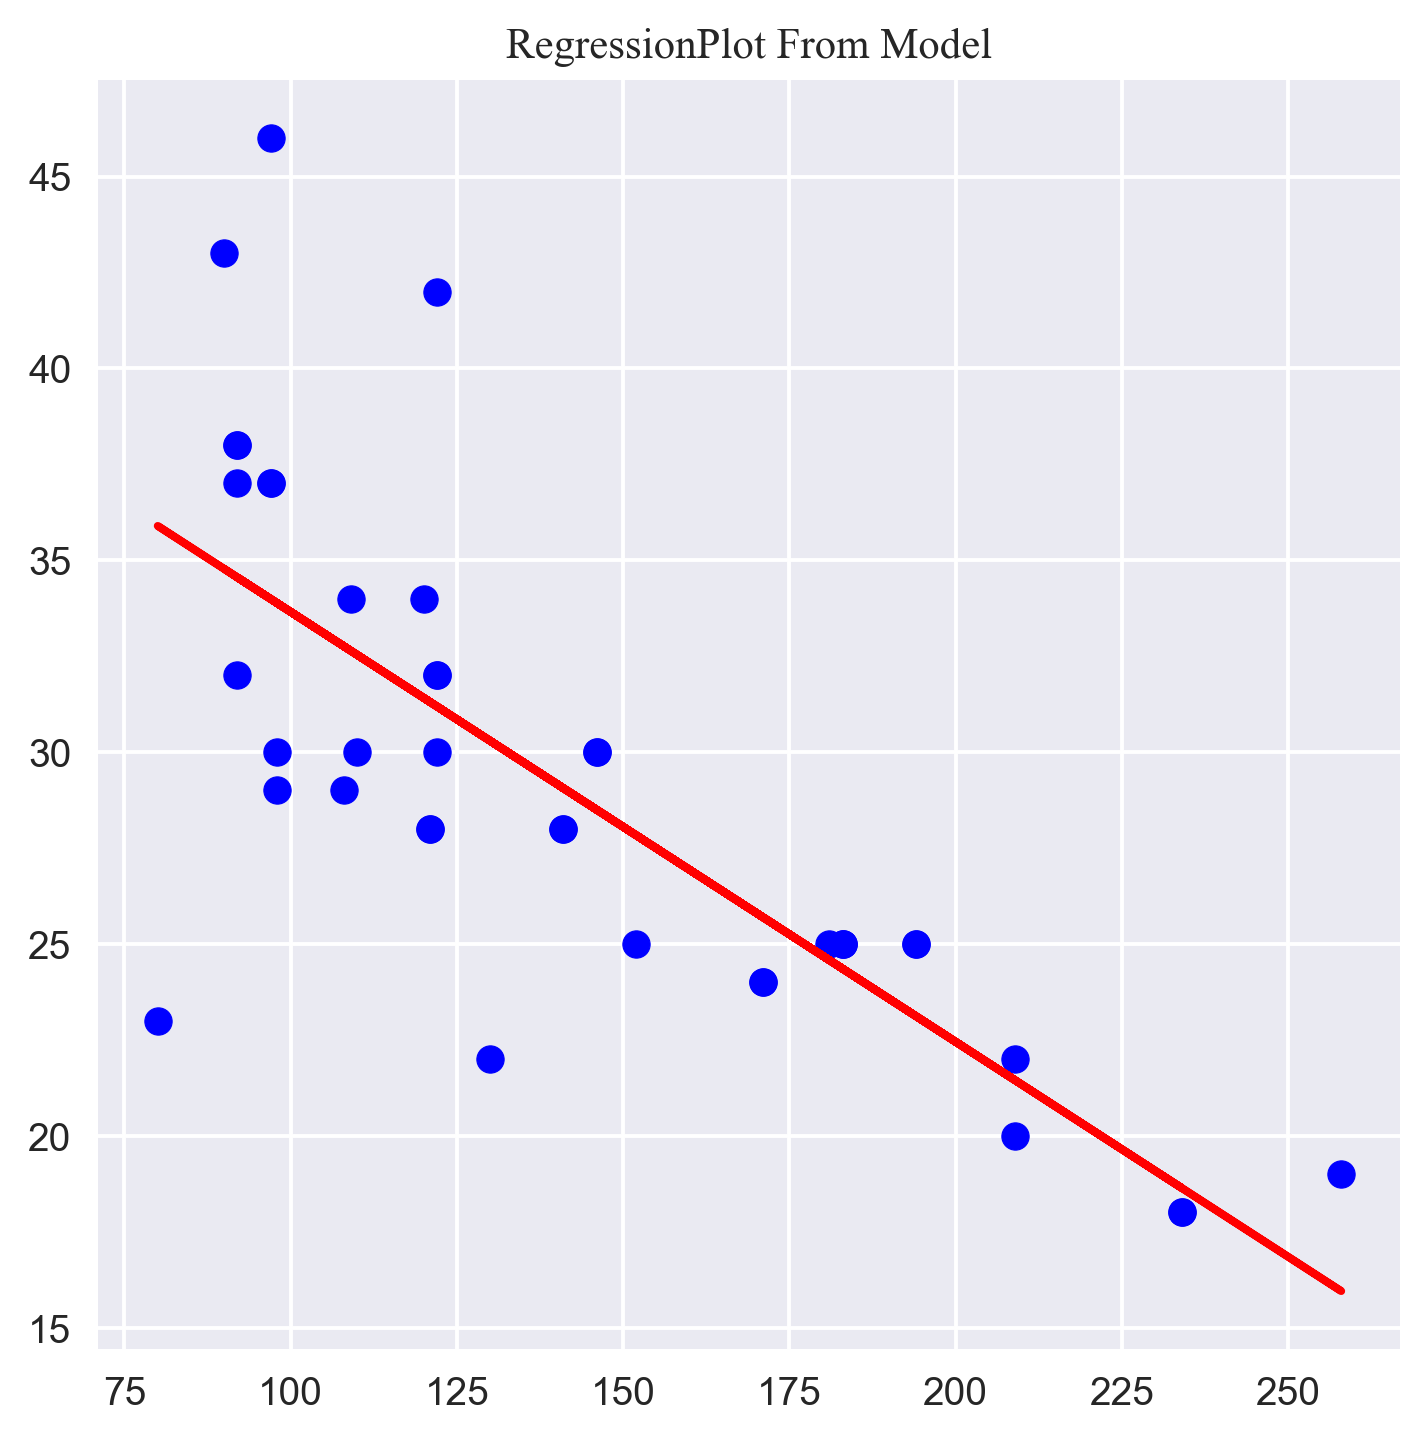
\includegraphics[width=\columnwidth]{images/plot_pred_test_set.png}
  \caption{Prediction Plot Engine size and Highway MPG}
  \label{fig:predplt}
\end{figure}
 
 
 There are few outliers. The regression model can also be compared with 
 the scatterplot for the whole data set
 in Figure~\ref{fig:scatterplt} as shown below, shows fairly show how data 
 points are aligned.
 
  \begin{figure}[h!]
  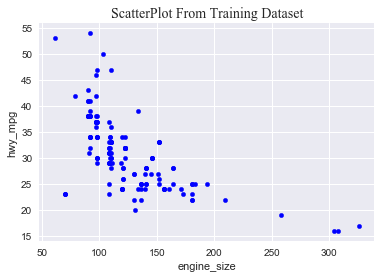
\includegraphics[width=\columnwidth]{images/scatterplot.png}
  \caption{Scatter Plot Engine size and Highway MPG}
\label{fig:scatterplt}
\end{figure} 
 
\section{Deploying App to Heroku} 

This service is tested using Dockerfile and Makefile and is able to fetch
output locally. Now, the application is tested in heroku cloud platform. Heroku
is chosen as the platform is open source as long as the application needs few 
`dyno', that is one or two. Which means as long as application has minimal
requirements. Dynos are containers provided by heroku platform where we can 
push our application and instruct them to execute the application.

Another reason of choosing heroku is that we do not have to worry about 
containers or nodes to scale up app deployment. Heroku manages all of these
needs. As an application developer, we just need to work on designing the 
intended app. For authentication an user account is created in heroku.com
using heroku dashboard.Then heroku command line is downloaded in local terminal.
Then run heroku login which in turn asks us to enter our email and password
for authentication.

As this project requires python's data analysis and machine-learning packages 
it is then deployed using Dockerfile. 

\subsection{Dockerfile and Heroku Container Registry}
 Our app named \textit{regressionAPI} needs several python packages. These
 packages can be added using heroku buildpacks. But for convenient deployment
 it is deployed using docker. Docker needs to be installed locally before 
 starting the process. Then `Dockerfile' is created  so that
 all of our required packages are fetched from it. Docker image is built from
 miniconda which comes with python, pandas, numpy and scipy. Using conda install
 scikit--learn, this package is also fetched into the 
 container~\cite{hid-sp18-415-dockerfile}.  

Now app is almost ready to be deployed to Heroku. The process needs
following three files.

\begin{itemize}
 \item A Dockerfile that helps with building a docker image and installing 
 all the dependencies or requirements for running Flask api in Heroku.
 To deploy Flask api using Dockerile, container has to be registered into 
 heroku by command. 
 \item Requirements.txt file~\cite{hid-sp18-415-regapp}
 \item Python files or application files. In this case regressionAPI.py
 \item wsgi.py file~\cite{hid-sp18-415-regapp}
 \item A Procfile that tells heroku what process to run. Here is an example 
 of Procfile \verb|web: gunicorn appname:app|. In this example web is a 
 process which tells heroku to run in the web and gunicorn handles requests
 and appname is name of our application which in our case is 
 regressionAPI~\cite{hid-sp18-415-regressionapi}.
 \end{itemize}
 
 Now we need to run following commands from local terminal.
 
 \verb|heroku container:login|~\cite{hid-sp18-415-heroku-com}. This registers
 our docker container to heroku. Then \verb|heroku create| creates app remotely
 into heroku and gives us app name from heroku
 Then to buildbuild image, push to Container Registry by command 

\begin{verbatim}
    heroku container:push web --app appname
\end{verbatim}

 and open the app in the browser herokuapp.com. With following
 command~\cite{hid-sp18-415-heroku-com}:

\begin{verbatim}
    heroku open --app appname
\end{verbatim}

 It launches app into heroku. By logging into heroku dashboard
 execution logs can be observed whcich helps debugging the whole
 process.
 
\section{Limitations and Challenges}
 
The project was intended also to do benchmarking by running rest services in
locally developed raspberry pi cluster. Three node pi cluster is created 
for the purpose with raspbian images on all of them. Certain issues in packages 
installations are the challenges at the moment.

\section{Conclusion}

REST services with flask is simple to develop and deploy. 
This project build a
simple regression model from car dataset. Regression plot and r square
value has been used to explain variance in miles per gallon (our dependent
variable). The model details is later used as 
a path for flask application. Also based on the model new data points can be 
used for future prediction. The application is successsfully run in localhost
with command python regressionAPI.py. Also deployed in heroku cloud platform 
using docker container. The whole project has been dockerized in
a docker container using Dockerfile. 




\begin{acks}

  The authors would like to thank Dr.~Gregor~von~Laszewski for his
  support and suggestions to write this paper and teaching assistants who
  helped me with all sorts of technical assistants.

\end{acks}



\bibliographystyle{ACM-Reference-Format}
\bibliography{report} 
